\subsection{uint256 Arithmetic Operations}\label{subsec:uint256-arithmetic-operation}

\subsubsection{ADD}

\emph{Library function interface:} \verb|uint256_add(uint256 a, uint256 b)|

\begin{enumerate}
    \item Split two uint256 inputs $a$ and $b$ into two parts of the upper 128 bits and the lower 128 bits, and perform Range Check.
    \item Perform field addition between the lower 128 bits of two numbers where reuse the constraints of field addition in Section \ref{subsec:field-arithmetic-constraints}, then we get the lower 128 bits of the uint256 result and the carry flag \verb|carry_lo|.
    \item Perform field addition between the upper 128 bits and add \verb|carry_lo|, then we get the upper 128 bits of uint256 and carry flag \verb|carry_hi|.
\end{enumerate}

The instructions corresponding to the addition of uint256 are
\begin{lstlisting}[language={}]
split128 r_a, r_a_lo, r_a_hi
split128 r_b, r_b_lo, r_b_hi
[r_src1] = [r_a_lo]
[r_src2] = [r_b_lo]
range_check(r_src1, MAX_uint128)
range_check(r_src2, MAX_uint128)
ADD r_dst_lo, r_src1, r_src2

if r_dst_lo >= 2^128:
    carry_lo = 1
    %{
        r_dst_lo = r_dst_lo - 2^128
    %}
else:
    carry_lo = 0

[r_src1] = [r_a_hi]
[r_src2] = [r_b_hi]
range_check(r_src1, MAX_uint128)
range_check(r_src2, MAX_uint128)
ADD r_dst_hi, r_src1, r_src2
[r_carry] = carry_lo
ADD r_dst_hi, r_dst_hi, r_carry

if r_dst_hi >= 2^128:
    carry_hi = 1
    %{
        r_dst_hi = r_dst_hi - 2^128
    %}
else:
    carry_hi = 0

[r_carry] = carry_hi
%{
    [r_dst] = [r_dst_hi] * 2^128 + [r_dst_lo]
%}
return [r_dst], [r_carry]
\end{lstlisting}

The corresponding constraints are
\begin{align*}
    & \texttt{r\_lo} \in [0,2^{128}), \\
    & \texttt{r\_hi} \in [0,2^{128}), \\
    & \texttt{carry\_lo} \cdot (\texttt{carry\_lo} - 1) = 0, \\
    & \texttt{carry\_hi} \cdot (\texttt{carry\_hi} - 1) = 0, \\
    & \texttt{dst\_lo} + \texttt{carry\_lo} \cdot 2^{128} - (\texttt{a\_lo} + \texttt{b\_lo}) = 0, \\
    & \texttt{dst\_hi} + \texttt{carry\_hi} \cdot 2^{128} - (\texttt{a\_hi} + \texttt{b\_hi}) = 0.
\end{align*}

\subsubsection{NOT}

\emph{Library function interface:} \verb|uint256_not(uint256 a)|

The instructions corresponding to bitwise NOT of uint256 are
\begin{lstlisting}[language={}]
split128 r_a, r_a_lo, r_a_hi
[r_src1] = [r_a_lo]
[r_src2] = [r_a_hi]
range_check(r_src1, MAX_uint128)
range_check(r_src2, MAX_uint128)
[r_u128] = 2^128 - 1
[r_dst_lo] = [r_u128] - [r_src1]
[r_dst_hi] = [r_u128] - [r_src2]
%{
    [r_dst] = [r_dst_hi] * 2^128 + [r_dst_lo]
%}
return [r_dst]
\end{lstlisting}

The corresponding constraints are
\begin{align*}
    & \texttt{r\_lo} \in [0, 2^{128}), \\
    & \texttt{r\_hi} \in [0, 2^{128}), \\
    & \texttt{[r\_dst\_lo]} + \texttt{[r\_a\_lo]} - 2^{128} + 1 = 0, \\
    & \texttt{[r\_dst\_hi]} + \texttt{[r\_a\_hi]} - 2^{128} + 1 = 0.
\end{align*}

\subsubsection{NEG}

\emph{Library function interface:} \verb|uint256_neg(uint256 a)|

The negation of uint256 relies on two uint256 operations, ADD and NOT, so the constraints of these two operations will also be used, but will not be enumerated again under this operation.
The corresponding instructions are
\begin{lstlisting}[language={}]
[r_not_num] = uint256_not(a)
[r_dst] = uint256_add(r_not_num, 1)
return [r_dst]
\end{lstlisting}

The corresponding constraint is
\[ \texttt{[r\_dst]} + \texttt{[r\_a]} - 2^{256} = 0. \]

\subsubsection{SUB}

\emph{Library function interface:} \verb|uint256_sub(uint256 a, uint256 b)|

The instructions corresponding to the subtraction of uint256 are
\begin{lstlisting}[language={}]
split128 r_a, r_a_lo, r_a_hi
split128 r_b, r_b_lo, r_b_hi
[r_src1] = [r_a_lo]
[r_src2] = [r_b_lo]
range_check(r_src1, MAX_uint128)
range_check(r_src2, MAX_uint128)

if r_src1 <= r_src2:
    borrow_lo = 0
else:
    borrow_lo = 1
    [r_u128] = 2^128
    add r_src1, r_src1, r_u128
SUB r_dst_lo, r_src1, r_src2

[r_src1] = [r_a_hi]
[r_src2] = [r_b_hi]
range_check(r_src1, MAX_uint128)
range_check(r_src2, MAX_uint128)
[r_borrow] = borrow_lo
ADD r_src2, r_src2, r_borrow

if r_src1 <= r_src2:
    borrow_hi = 0
else:
    borrow_hi = 1
    [r_u128] = 2^128
    ADD r_src1, r_src1, r_u128
SUB r_dst_hi, r_src1, r_src2

[r_borrow] = borrow_hi
%{
    [r_dst] = [r_dst_hi] * 2^128 + [r_dst_lo]
%}
return [r_dst], [r_borrow]
\end{lstlisting}

The corresponding constraints are
\begin{align*}
    & \texttt{r\_lo} \in [0, 2^{128}), \\
    & \texttt{r\_hi} \in [0, 2^{128}), \\
    & \texttt{carry\_lo} \cdot (\texttt{carry\_lo} - 1) = 0, \\
    & \texttt{carry\_hi} \cdot (\texttt{carry\_hi} - 1) = 0, \\
    & \texttt{dst\_lo} + \texttt{borrow\_lo} \cdot 2^{128} - (\texttt{a\_lo} + \texttt{b\_lo}) = 0, \\
    & \texttt{dst\_hi} + \texttt{borrow\_hi} \cdot 2^{128} - (\texttt{a\_hi} + \texttt{b\_hi}) = 0.
\end{align*}

\subsubsection{MUL}

\emph{Library function interface:} \verb|uint256_mul(uint256 a, uint256 b)|

The range of the multiplication result of two uint256 numbers is $[0,2^{512})$, so the final result needs to be stored in two registers and the numbers are splitted into 128 bits for multiplication and addition in calculation process. The principle is as Figure \ref{fig:u256-mul}.
\begin{figure}[!htp]
    \centering
    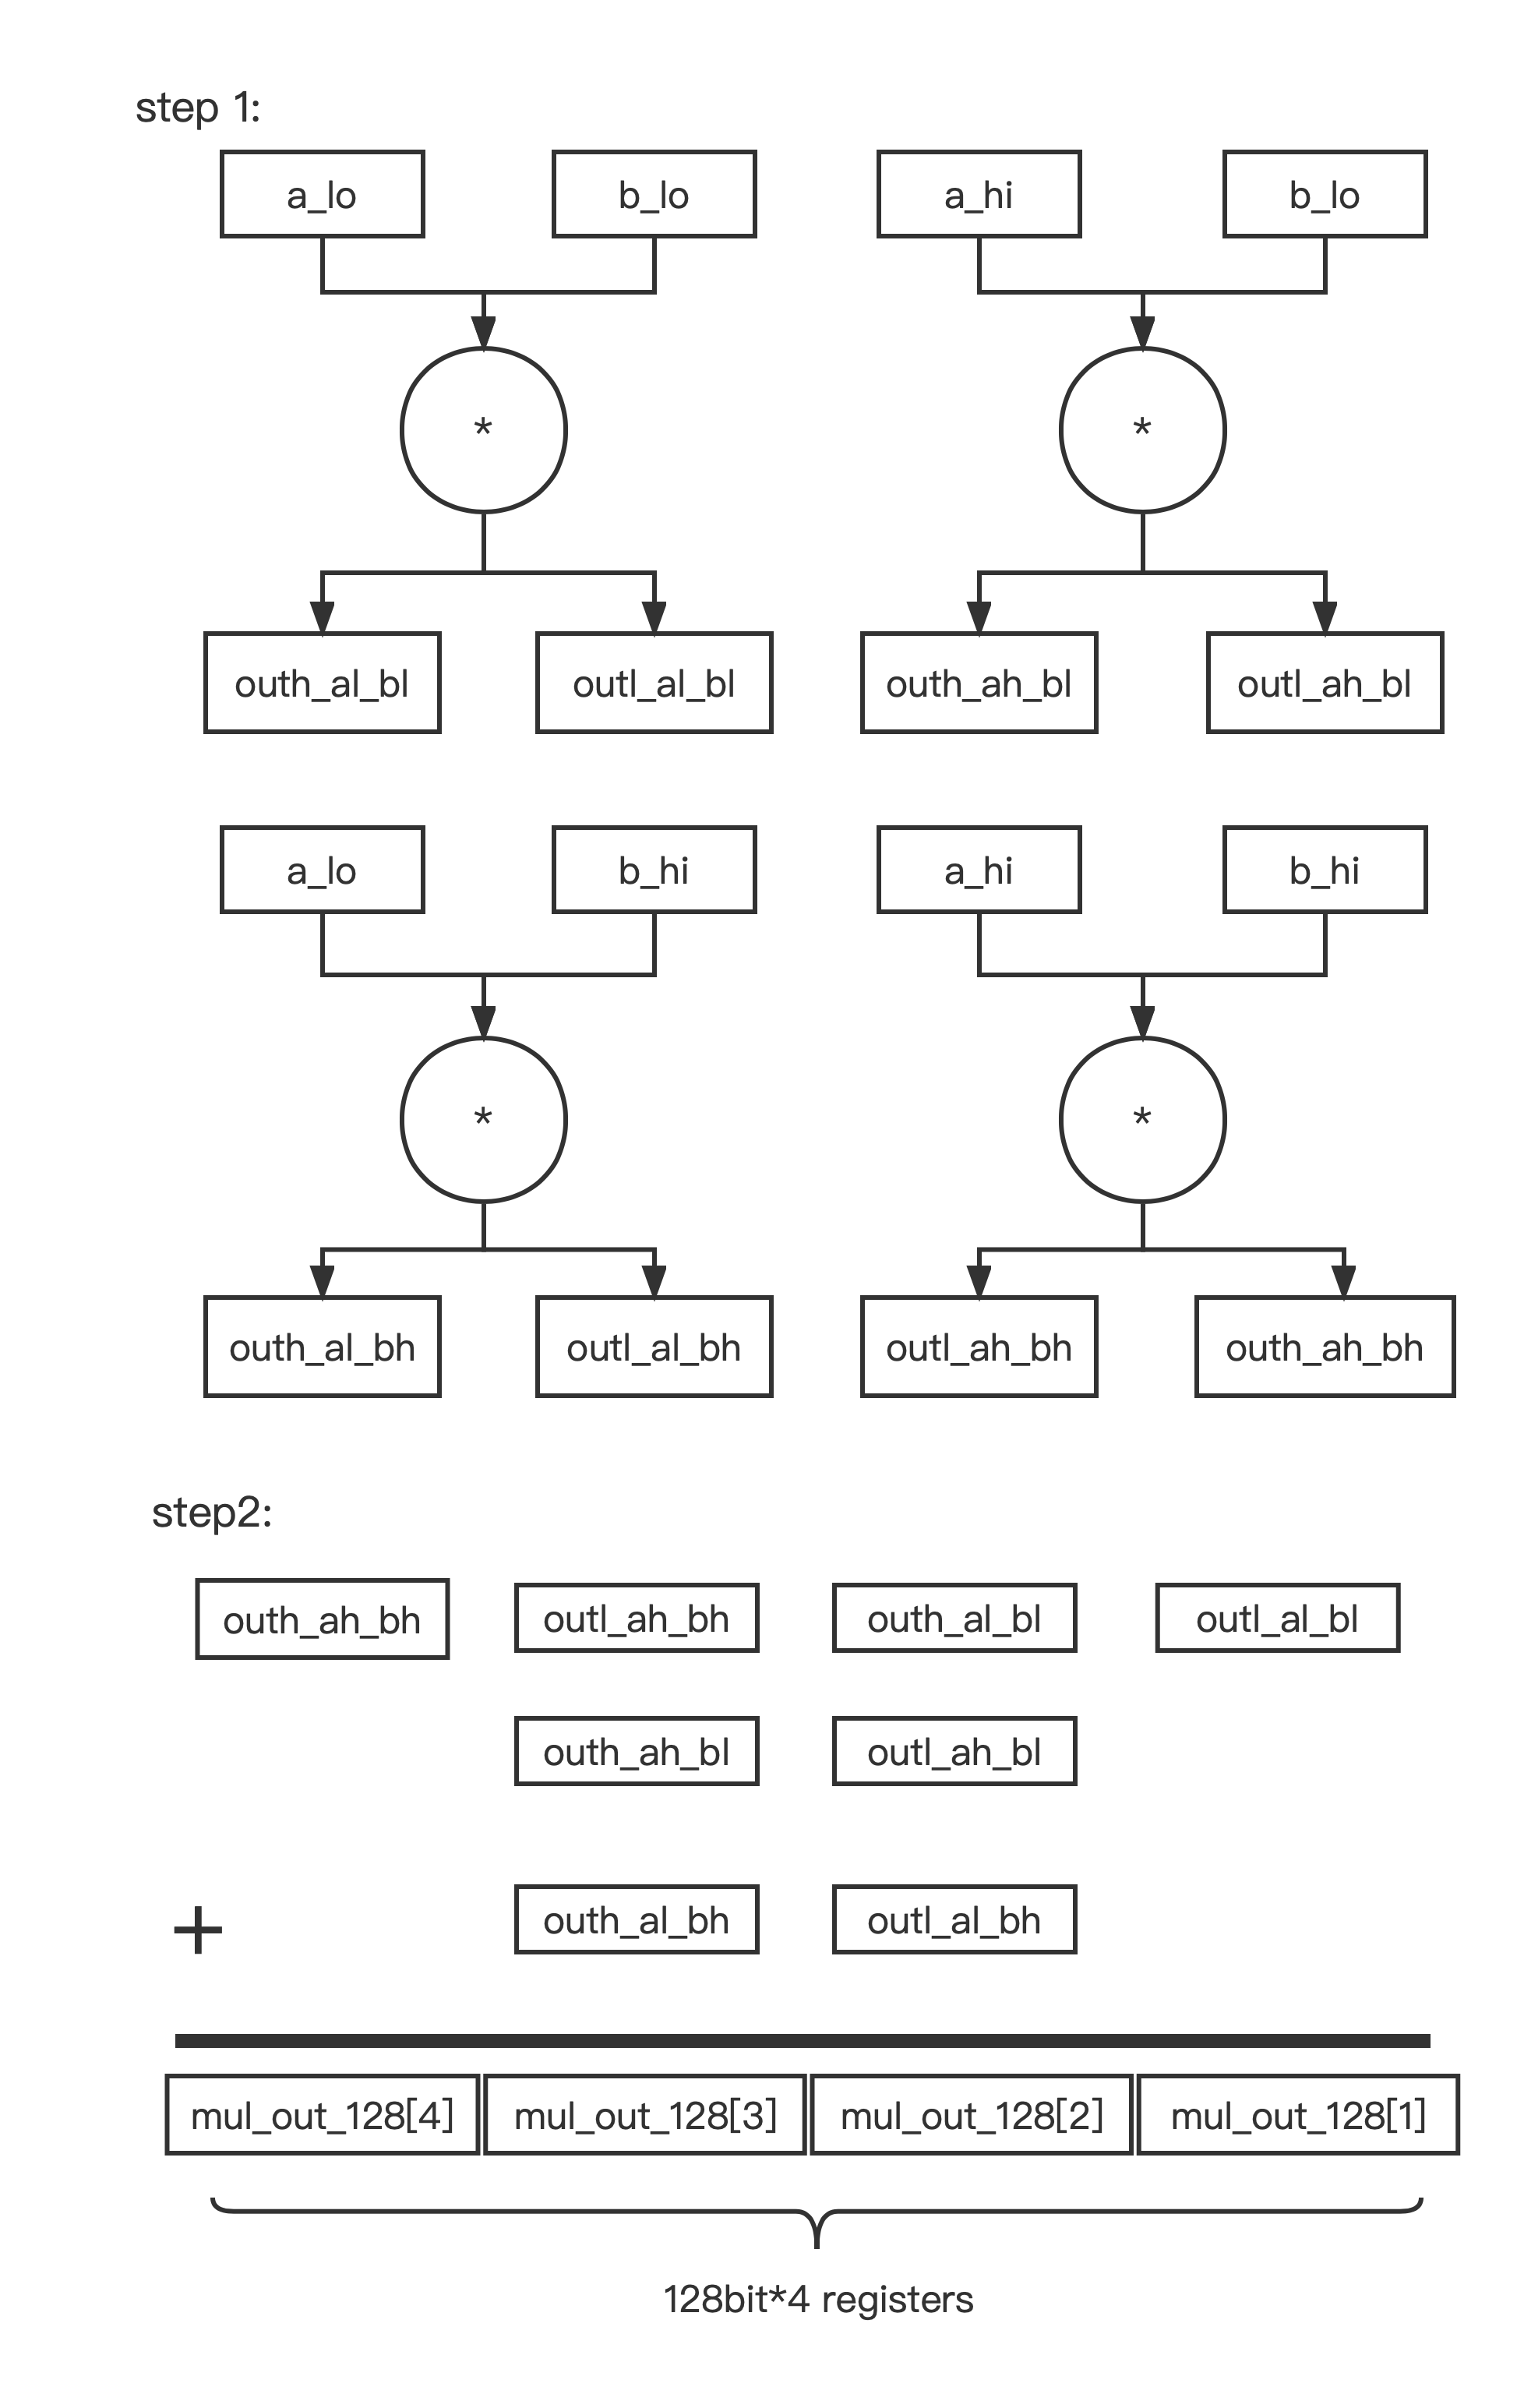
\includegraphics[width=0.8\textwidth]{u256-mul.png}
    \caption{uint256 multiplication algorithm}
    \label{fig:u256-mul}
\end{figure}

The instructions corresponding to the multiplication of uint256 are
\begin{lstlisting}[language={}]
split128 r_a, r_a_lo, r_a_hi
split128 r_b, r_b_lo, r_b_hi
[r_src1] = [r_a_lo]
[r_src2] = [r_b_lo]
range_check(r_src1, MAX_uint128)
range_check(r_src2, MAX_uint128)
MUL r_dst_al_bl, r_src1, r_src2

[r_src1] = [r_a_hi]
[r_src2] = [r_b_lo]
range_check(r_src1, MAX_uint128)
range_check(r_src2, MAX_uint128)
MUL r_dst_ah_bl, r_src1, r_src2

[r_src1] = [r_a_lo]
[r_src2] = [r_b_hi]
range_check(r_src1, MAX_uint128)
range_check(r_src2, MAX_uint128)
MUL r_dst_al_bh, r_src1, r_src2

[r_src1] = [r_a_hi]
[r_src2] = [r_b_hi]
range_check(r_src1, MAX_uint128)
range_check(r_src2, MAX_uint128)
MUL r_dst_ah_bh, r_src1, r_src2

split128 r_dst_al_bl, r_dst_al_bl_lo, r_dst_al_bl_hi
split128 r_dst_ah_bl, r_dst_ah_bl_lo, r_dst_ah_bl_hi
split128 r_dst_al_bh, r_dst_al_bh_lo, r_dst_al_bh_hi
split128 r_dst_ah_bh, r_dst_ah_bh_lo, r_dst_ah_bh_hi

range_check(r_dst_al_bl_hi, MAX_uint128)
range_check(r_dst_ah_bl_lo, MAX_uint128)
[r_mul_out_128_1] = [r_dst_al_bl]

ADD r_mul_out_128_2, r_dst_al_bl_hi, r_dst_al_bl_hi
ADD r_mul_out_128_2, r_mul_out_128_2, r_dst_al_bh_lo

split128 r_mul_out_128_2, r_mul_out_128_2, r_mul_out_128_2_carry

ADD r_mul_out_128_3, r_mul_out_128_2_carry, r_dst_ah_bl_hi
ADD r_mul_out_128_3, r_mul_out_128_3, r_dst_al_bh_hi
ADD r_mul_out_128_3, r_mul_out_128_3, r_dst_ah_bh_lo

split128 r_mul_out_128_3, r_mul_out_128_3, r_mul_out_128_3_carry

ADD r_mul_out_128_4, r_mul_out_128_3_carry, r_dst_ah_bh_hi

%{
    r_mul_out_256_2 = r_mul_out_128_4 * 2^128 + r_mul_out_128_3
    r_mul_out_256_1 = r_mul_out_128_2 * 2^128 + r_mul_out_128_1
%}

return [r_mul_out_256_2], [r_mul_out_256_1]
\end{lstlisting}

The multiplication of uint256 is composed of several instructions. The instructions are constrained by corresponding constraints in Section \ref{subsec:field-arithmetic-constraints}. The independent constraint of multiplication is
\[ \texttt{[r\_mul\_out\_256\_2]} \cdot 2^{256} + \texttt{[r\_mul\_out\_256\_1]} - \texttt{a} \cdot \texttt{b} = 0. \]

\subsubsection{DIV}

\emph{Library function interface:} \verb|uint256_div(uint256 a, uint256 div)|

The instructions corresponding to the division of uint256 are
\begin{lstlisting}[language={}]
if div == 0:
    return 0, 0
%{
    quotient = a / div
    remainder = a % div
%}
[r_quotient] = quotient
(r_mul_out_256_2, r_mul_out_256_1) = uint256_mul(r_quotient, div)
[r_zero] = 0
EQ r_mul_out_256_2, r_zero

[r_rem] = remainder

(r_a_check, r_add_carry) = uint256_add(r_mul_out_256_1, r_rem)
EQ r_a_check, r_a
EQ r_add_carry, r_zero
return [r_quotient], [r_rem]
\end{lstlisting}

The division of uint256 is composed of several instructions. The instructions are constrained by corresponding constraints in Section \ref{subsec:field-arithmetic-constraints}. The independent constraint of division is
\[ \texttt{[r\_quotient]} \cdot \texttt{[r\_div]} + \texttt{[r\_rem]} - \texttt{[r\_a]} = 0. \]
